\chapter{New "generation" of tools}

This chapter describes some new tools, probably their documentation will be reoargnized once they are completely stabilized.


%-------------------------------------------------------------------
%-------------------------------------------------------------------

\section{Fully automatic dense matching}

\subsection{Generalities}

The {\tt C3CD} command is the command that compute automatically a point cloud from a set of oriented images.

\begin{verbatim}
mm3d C3DC -help
Valid types for enum value:
   Ground
   Statue
   TestIGN
   QuickMac
*****************************
*  Help for Elise Arg main  *
*****************************
Mandatory unnamed args :
  * string :: {Type in enumerated values}
  * string :: {Full Name (Dir+Pattern)}
  * string :: {Orientation}
Named args :
  * [Name=Masq3D] string :: {3D masq for point selection}
  * [Name=Out] string :: {final result (Def=C3DC.ply)}
  * [Name=SzNorm] INT :: {Sz of param for normal evaluation (<=0 if none, Def=2 mean 5x5) }
  * [Name=PlyCoul] bool :: {Colour in ply ? Def = true}
  * [Name=Tuning] bool :: {Will disappear soon ...}
\end{verbatim}


The syntax is :

\begin{itemize}
  \item type of matching in enumerated values,

  \item set of images to use

  \item orientation

  \item if {\tt Masq3D} is specified, indicates a 3D masq as created with {\tt SaisieMasqQT};
  \item if {\tt SzNorm} is specified, indicates the window size parameters for normal extraction in ply file
        (usefull for meshing);
  \item if {\tt PlyCoul} is specified, indicates that colouring of points is required.
\end{itemize}


\subsection{Quickmac option}

The {\tt QuickMac} uses the {\tt MMInitialModel} as matcher, which is quite fast on CPU.
As example we use a dataset of $41$ images of a statue, they are presented on figure~\ref{FIG:Angel:Flog}.


\begin{figure}
\begin{center}
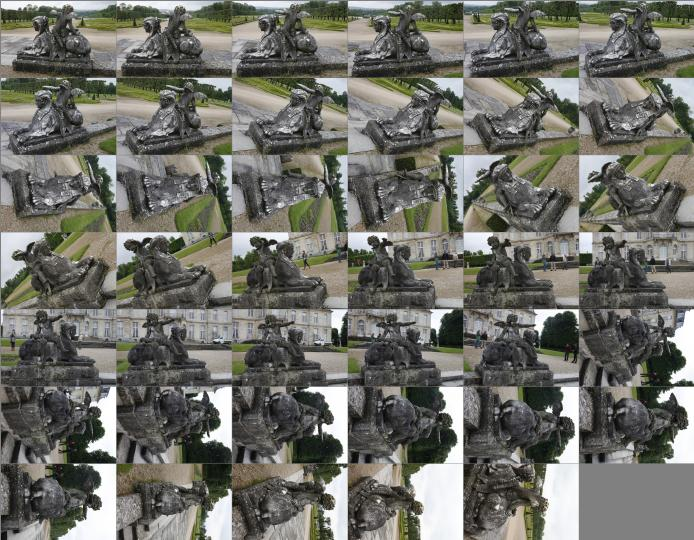
\includegraphics[width=120mm]{FIGS/Ange/Panel.jpg}
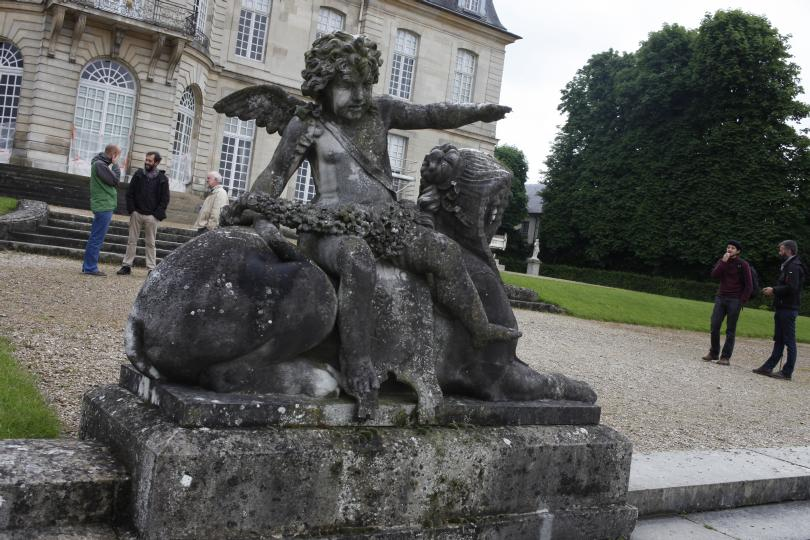
\includegraphics[width=120mm]{FIGS/Ange/SMALL_MG_1044.JPG}
\end{center}
\caption{The Angel'statue used for the {\tt C3DC QuickMac} command}
\label{FIG:Angel:Flog}
\end{figure}


Here is a possible command using a dataset of $41$ images of a statue :


\begin{verbatim}
mm3d C3DC QuickMac _MG_10.*JPG Ori-All2/ Masq3=AperiCloud_All2_selectionInfo.xml
\end{verbatim}


The result are presented on figure~\ref{FIG:Angel:Result}. Computation time was $12$ min with a $8$ processor machine.




\begin{figure}
\begin{center}
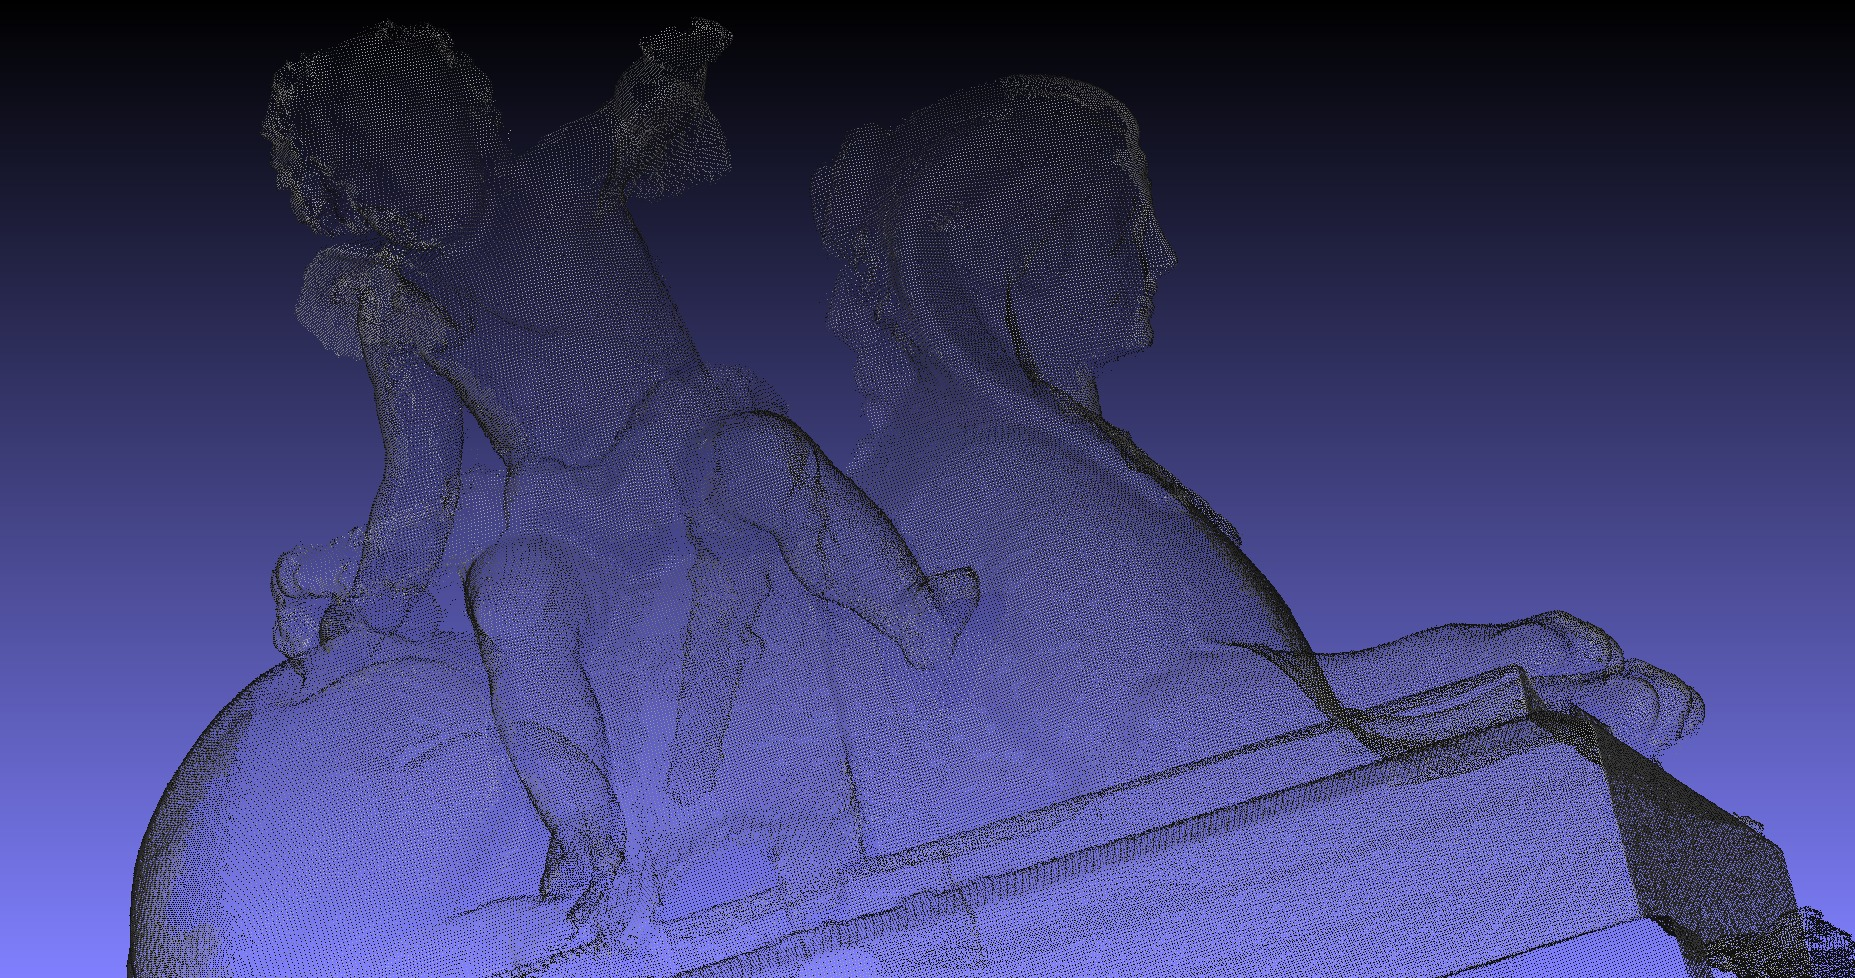
\includegraphics[width=100mm]{FIGS/Ange/snapshot00.jpg}
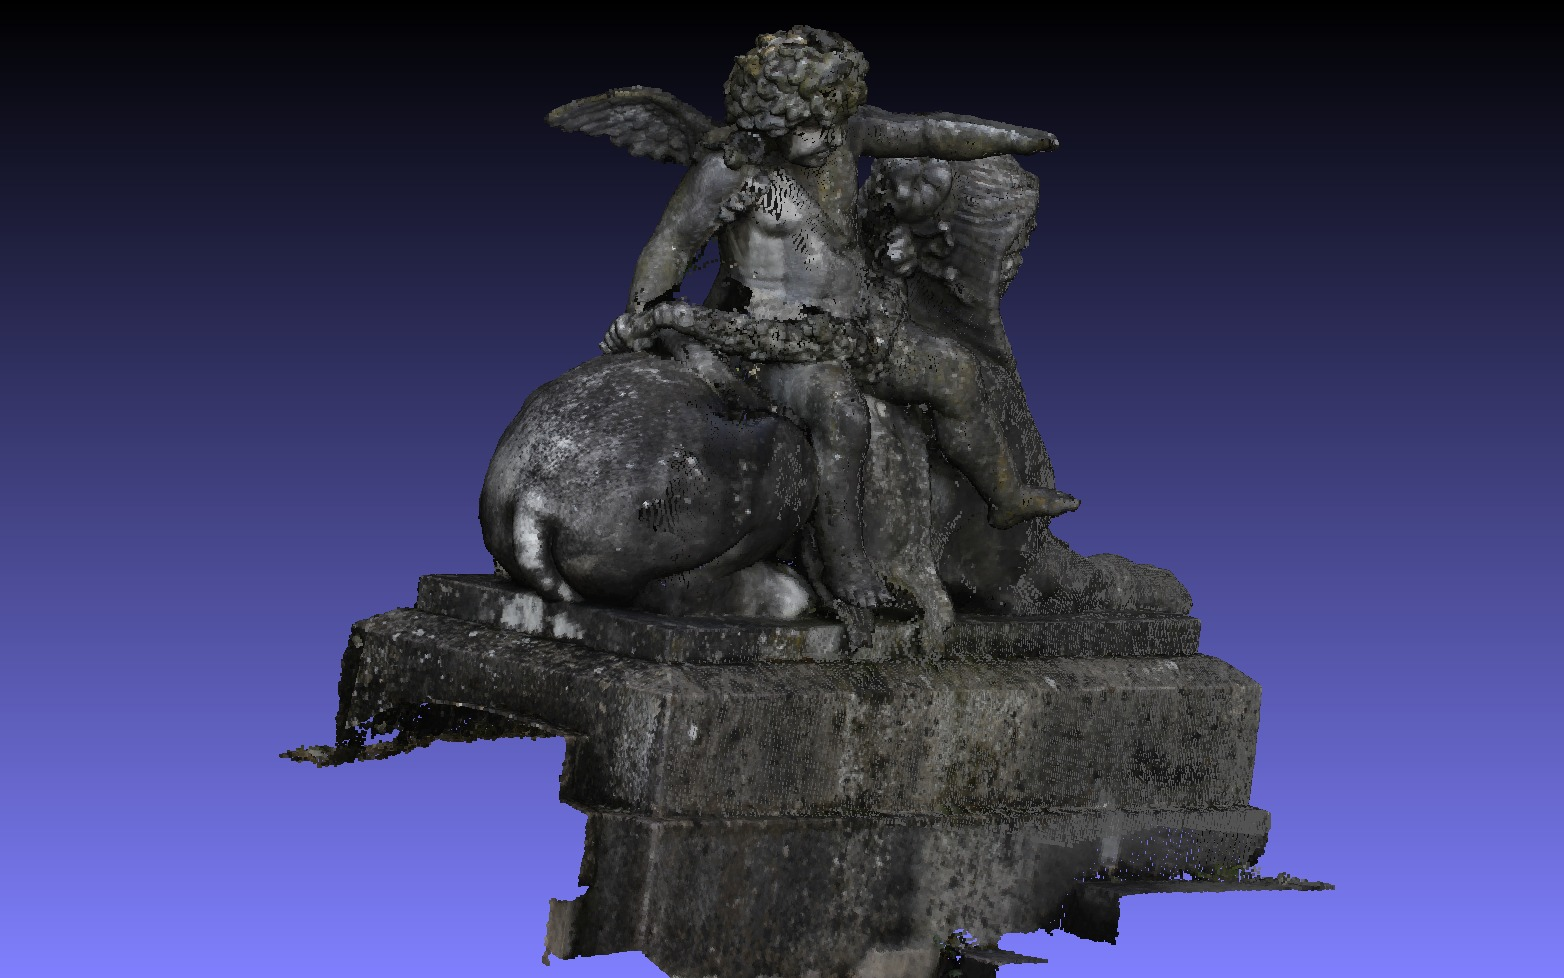
\includegraphics[width=100mm]{FIGS/Ange/snapshot01.jpg}
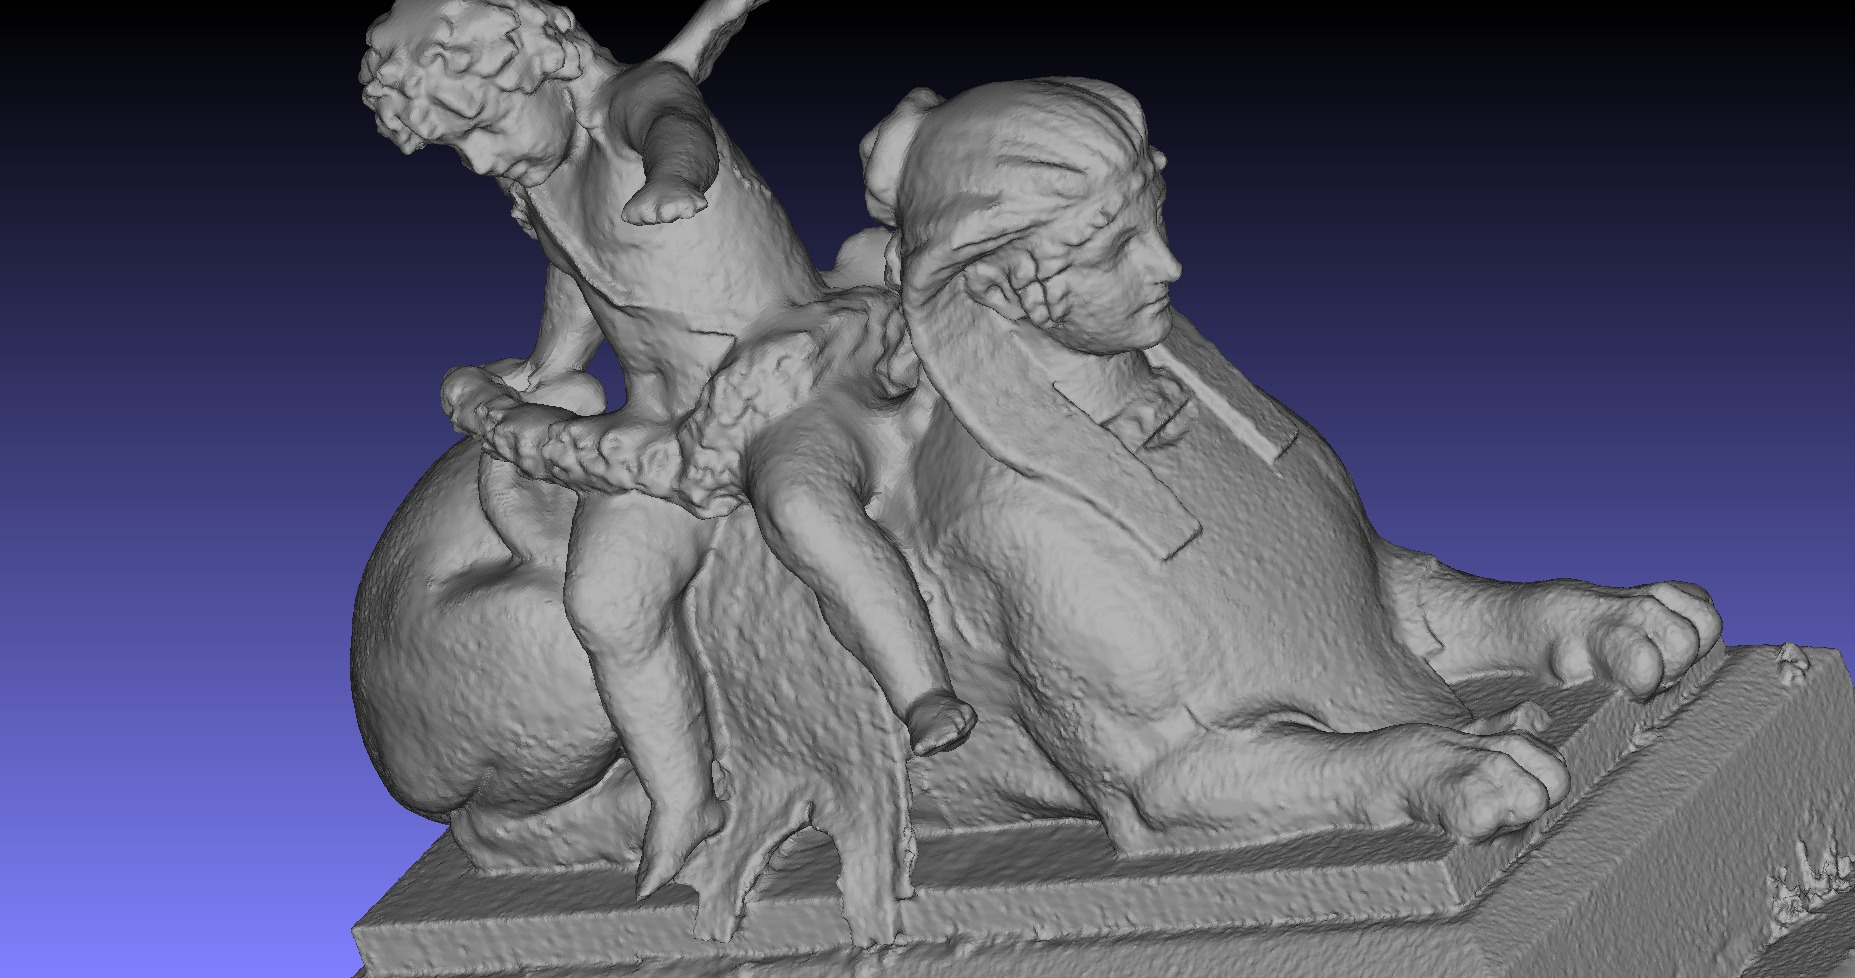
\includegraphics[width=100mm]{FIGS/Ange/snapshot201.jpg}
\end{center}
\caption{Result of {\tt C3DC QuickMac} command: point cloud, coloured point cloud, meshed poind cloud}
\label{FIG:Angel:Result}
\end{figure}

%-------------------------------------------------------------------
%-------------------------------------------------------------------

\section{Parallelizing Apero}

For now works only with linear orientation.

\subsection{Parallelizing Apero}

The new tool {\tt Liquor} (for LInear QUick ORientation) accelerate the computation of orientation. The acceleration comes
from two aspects:

\begin{itemize}
   \item  it uses a hierarchical building of orientation, which make the computation in $N Log N$ instead of $N^2$
   \item  at the low level of the pyramid, it parallelizes the computation of subset on the several processors.
\end{itemize}

The syntax :

\begin{verbatim}
mm3d Liquor -help
*****************************
*  Help for Elise Arg main  *
*****************************
Mandatory unnamed args :
  * string :: {Full name (Dir+Pat)}
  * string :: {Caliibration Dir}
Named args :
  * [Name=SzInit] INT :: {Sz of initial interval (Def=50)}
  * [Name=OverLap] REAL :: {Prop overlap (Def=0.1) }
\end{verbatim}

An example of use with the data set of figure~\ref{FIG:Liquor:DataMap} :

\begin{verbatim}
mm3d Liquor CAM2_0.* Ori-Calib/
\end{verbatim}


With these $150$ images the computation time is $20 min$ instead of $1h10min$ with traditional {\tt Tapas}.

\begin{figure}
\begin{center}
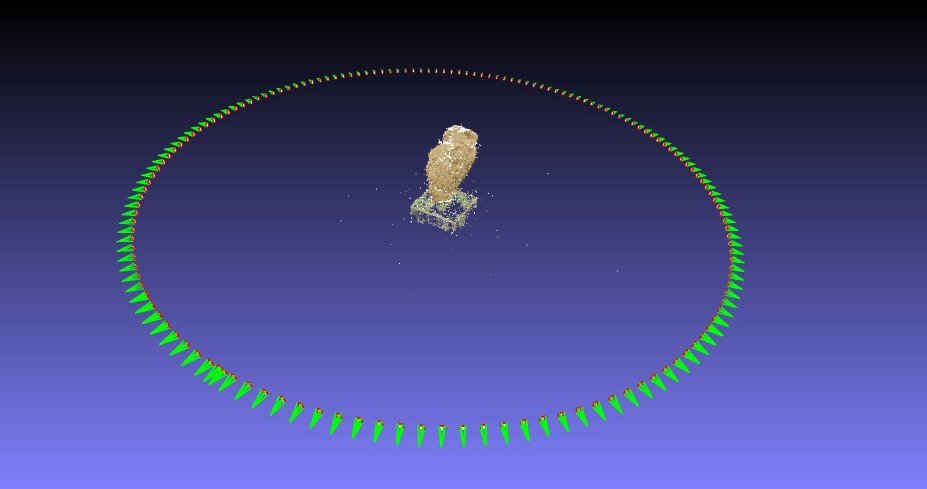
\includegraphics[width=100mm]{FIGS/Ange/LineAcq.jpg}
\end{center}
\caption{Linear acquisition used for {\tt Liquor} command}
\label{FIG:Liquor:DataMap}
\end{figure}


